\documentclass{article}%
\usepackage[T1]{fontenc}%
\usepackage[utf8]{inputenc}%
\usepackage{lmodern}%
\usepackage{textcomp}%
\usepackage{lastpage}%
\usepackage[head=40pt,margin=0.5in,bottom=0.6in]{geometry}%
\usepackage{graphicx}%
%
\title{\textbf{La feminización del VIH en Venezuela sumergida en una crisis}}%
\author{EFE}%
\date{26/09/2018}%
%
\begin{document}%
\normalsize%
\maketitle%
\textbf{URL: }%
http://www.el{-}nacional.com/noticias/salud/feminizacion{-}del{-}vih{-}venezuela{-}sumergida{-}una{-}crisis\_253363\newline%
%
\textbf{Periodico: }%
EN, %
ID: %
253363, %
Seccion: %
Salud\newline%
%
\textbf{Palabras Claves: }%
Salud, Crisis humanitaria\newline%
%
\textbf{Derecho: }%
2.1%
, Otros Derechos: %
NO\_TIENE%
, Sub Derechos: %
2.1.1%
\newline%
%
\textbf{EP: }%
NO\newline%
\newline%
%
\textbf{\textit{La mujer con VIH suele ser estigmatizada o discriminada, pese a que la legislación le garantiza protección especial}}%
\newline%
\newline%
%
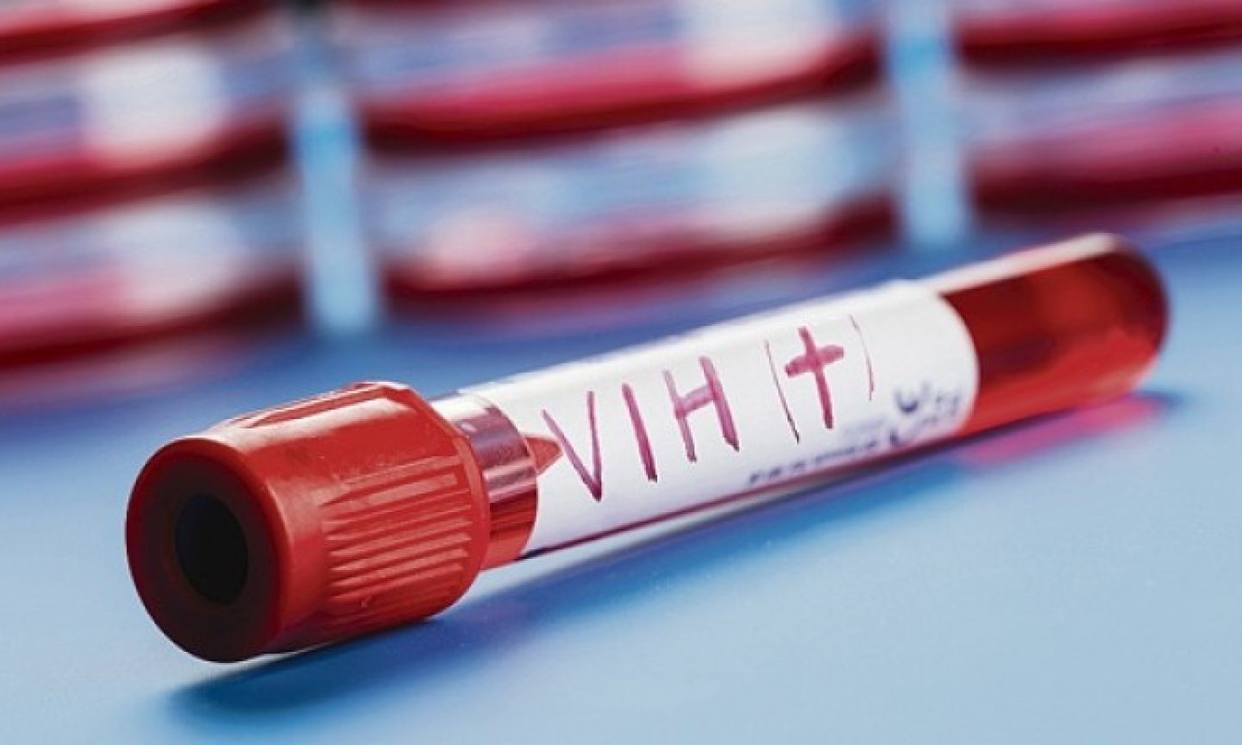
\includegraphics[width=300px]{93.jpg}%
\newline%
%
El Virus de Inmunodeficiencia Humana (VIH) afecta cada vez a más mujeres en Venezuela, país con una crisis económica que se traduce en escasez de tratamientos, depauperación de los hospitales y falta de información oficial sobre la enfermedad.%
\newline%
%
Actualmente ONU{-}SIDA estima que unas 120.000 personas viven en Venezuela con este virus, lo que no significa que todos lo sepan, pues registros oficiales ubican entre 71.000 y 77.000 individuos que reciben tratamientos antirretrovirales que el Estado entrega de manera gratuita.%
\newline%
%
Regina López,~representante de esta agencia de Naciones Unidas en Venezuela,~dijo a~Efe~que no hay certeza en los datos de los últimos dos años, razón por la que el informe mundial de la ONU de 2018 no incluyó un balance del país.%
\newline%
%
58 \% de las nuevas infecciones en todo el mundo fueron en mujeres, por lo que la feminización del virus es una tendencia global, de acuerdo con lo señalado en el informe.%
\newline%
%
La especialista señaló la imposibilidad de hacer diagnósticos en algunos hospitales y la escasez de antirretrovirales como dos problemas en Venezuela.%
\newline%
%
Tanto la funcionaria de la ONU como la infectóloga venezolana Graciela López, que trabaja en un hospital pediátrico de Caracas, consideran que la mujer con VIH es "estigmatizada" o "discriminada" pese a que la legislación local le garantiza una protección especial.%
\newline%
%
Estas mujeres deben sortear como el resto de ciudadanos la escasez de alimentos y fármacos que impera en el país y, en cientos de casos, atender a sus hijos que contrajeron el virus por la falta de atención óptima durante el embarazo y el parto.%
\newline%
%
La infectóloga explicó a~Efe~que la transmisión del virus a neonatos es prevenible, pero en el caso venezolano hay embarazadas con VIH que no están tomando tratamientos o están pariendo en vez de cesárea y, además, los hospitales no tienen fórmulas lácteas para estos recién nacidos.%
\newline%
%
"Estamos quitándoles la oportunidad de nacer sin virus y le estamos dando 30 \% de riesgo de nacer infectados", subrayó.%
\newline%
%
Mientras tanto, la intermitencia de los tratamientos ha sido denunciada en los últimos meses por los venezolanos que son seropositivos, muchos de los cuales han hecho pública en las redes sociales su preocupación por la falta de medicamentos que, alertan, pone en peligro sus vidas.%
\newline%
%
La Red Venezolana de Gente Positiva, que agrupa a todas las personas que viven con VIH, asegura que unas 3.000 personas murieron en el primer semestre del año producto del sida y sus enfermedades oportunistas, lo que arroja un aumento del 50 \% en la tasa de mortalidad que ellos manejan respecto al año pasado.%
\newline%
%
Eduardo Franco, secretario de la organización, aseguró a~Efe~que ha habido meses con "100 \% de desabastecimiento" en cuanto a los canales regulares y sin ningún tipo de respuesta~gubernamental.%
\newline%
%
Señaló que han recibido medicamentos~ por cooperación internacional; sin embargo, es insuficiente, pues compañeros han fallecido por la falta de medicamentos antirretrovirales.%
\newline%
%
Franco criticó la falta de información y aseveró que son unos 85.000 los inscritos en los programas oficiales para recibir el tratamiento pero cree que hay más de 300.000 personas que requieren medicamentos en Venezuela, que viven con VIH.%
\newline%
%
Denunció que los laboratorios del sistema de salud público no cuentan con los químicos para diagnosticar el virus, lo que estimula la ausencia de datos certeros, pero la red estima que si se hiciese una prueba "nacional" la cifra de infectados se ubicaría en 1 millón, muy por encima de la prevalencia que estima ONU en 0,6 \% (cerca de 200.000).%
\newline%
%
\end{document}